%Add a more informatic name
\chapter{Tools and platforms for reproducibility evaluations of neuroimaging pipelines}\label{toolsandplatforms}
%Intro 

%\todo{A few sentences of introduction to outline the chapter}
The tools and platforms used for the reproducibility evaluations of 
neuroinformatics pipelines are discussed in this chapter.
\todo{The rest of this paragraph is irrelevant. You should just describe the outline of the chapter here.}
The 
neurogimaging pipelines discussed here are mainly the preprocessing 
pipelines used for removing the noise from the neuroimaging data. For 
the ease of conducting the experiment and for the reproducibility, 
neuroimaging pipelines were containerized. The experiments were 
repeated several times under different conditions. We made use of a web 
platform (CBRAIN) for managing the containers and data. To find out the 
cause of the reproducibility issues, interposition techniques were used 
for the provenance capture.

\section{Neuroimaging Pipelines}\label{neuroimaging}
%What is neuroimagaing
%Check first sentence
Neuroimaging pipelines are used for the analysis and visualization of human brain structure, function and connectivity. Neuroscientists are relying on the neuroimaging techniques as an essential tool for understanding the complex spatial and temporal characteristics of human brain. Some popular neuroimaging techniques are functional magnetic resonance imaging (fMRI), diffusion tensor imaging (DTI), voxel based morphometry (VBM), magnetoencephalography (MEG), electroencephalography (EEG), and optical imaging. According  to the Handbook of Clinical Neurology~\cite{BUCHBINDER201661} fMRI, ``maps the spatiotemporal distribution of neural activity in the brain under varying cognitive conditions". DTI is defined in~\cite{Rizea11} as, ``a magnetic resonance imaging technique that enables the measurement of the diffusion of water in tissue in order to produce neural tract images". VBM according to Melonakos and et al.~\cite{MELONAKOS201165} is, ``a hypothesis-free, whole-brain, voxel-by-voxel analytic method that attempts to compare imaging data between populations". MEG is given a simple explanation in~\cite{Sato1985} as, ``the recording of magnetic fields generated by the brain". Brief description given for EEG in~\cite{Light2010} is, ``EEG measures the electrical activity of large, synchronously firing populations of neurons in the brain with electrodes placed on the scalp". The definition for optical imaging according to~\cite{doi:10.1080/23273798.2017.1290810} is, ``Optical imaging involves shining light into a tissue with one or more sources, and measuring light output from the tissue using one or more detectors".

%What is fMRI.
Among the neuroimaging techniques listed above, fMRI became so popular among neuroscientists due to the noninvasive nature of experiments, high temporal and spatial resolution, ease of implementation and high quality signal~\cite{Bandettini2009}. fMRI images can be used to identify the cerebral blood flow and oxygenation changes due to sensory, motor or cognitive tasks. The technique used by the fMRI technology relies on the blood oxygenated level-dependant (BOLD) method. The oxygenated and de-oxygenated hemoglobin have different magnetic characteristics and the change in the blood oxygenation level after a neuronal activity results in MRI signals~\cite{doi:10.1177/0883073807313047}. This change of oxygen levels in blood is the principle behind the BOLD-fMRI technology. BOLD-fMRI uses task-fMRI and resting-state fMRI for studying functional connectivity in human brain. Task-related fMRI analyses helps in identifying the functionally distinct nodes in the human brain belonging to a specific task~\cite{task_fmri} and resting-state fMRI helps in analyzing functional connectivity while the subject is at the state of rest~\cite{SMITH2013144}.

%Tools used for fMRI analysis
In neuroimaging, relevant information has to be extracted from noisy images of the brain~\cite{WOOLRICH2009S173}. To help extraction of structural, functional or diffusion MRI data, there are several pipelines freely available. Some of the most popular pipelines are The FMRIB Software Library\footnote{\url{https://fsl.fmrib.ox.ac.uk/fsl/fslwiki}} (FSL), FreeSurfer\footnote{\url{https://surfer.nmr.mgh.harvard.edu/}} and HCP Pipelines\footnote{\url{https://github.com/Washington-University/Pipelines}}.
 
%Add more details
\todo{Rewrite the following sentence so that you don't have to have quotes}
FSL~\cite{JENKINSON2012782}, ``is a comprehensive library of analysis tools for FMRI, MRI and DTI brain imaging data". This toolbox consists of over 230 individual command line tools and 23 GUIs, among which only a sub-set is commonly used. Table \ref{tab:tools_fsl} lists the most popular FSL tools. fMRI pre-processing can be implemented from FSL tools, for both task-based and resting-state fMRI. Among other things, FSL can do motion correction, distortion correction, spatial smoothing, temporal filtering and registration of images.

\todo{Rewrite the following sentence so that you don't have to have quotes}
According to~\cite{freesurfer_website}, ``FreeSurfer is a software package for the analysis and visualization of structural and functional neuroimaging data from cross-sectional or longitudinal studies". It consists of a set of tools that provide automated analysis of main features of human brain. The main tasks include volumetric segmentation, hippocampal subfield segmentation, inter-subject alignment based on the folding pattern of cortex, cortical gray matter thickness detection and human cerebral cortex surface model construction~\cite{Fischl2012}. 

\begin{center}
\tabulinesep=1.2mm
\begin{tabu} to \textwidth { | X[l] | X[l] | }
  \hline
  Use & Tool name \\
  \hline
  FMRI: task-based & FEAT \\
  \hline
  FMRI: resting-state or task-based & MELODIC \\
  \hline
  ASL (perfusion imaging of flow) & FABBER \\
  \hline
  Diffusion: probabilistic tractography & FDT \\
  \hline
  Diffusion: multi-subject voxel-wise analysis & TBSS \\
  \hline
  Brain extraction & BET \\
  \hline
  Tissue-type segmentation  & FAST \\
  \hline
  Subcortical segmentation & FIRST \\
  \hline
  Linear and Non-Linear Registration & FLIRT and FNIRT \\
  \hline
  Voxel-wise analysis of grey matter density & FSL-VBM \\
  \hline
  Whole brain atrophy (longitudinal and cross-sectional) & SIENA and SIENAX \\
  \hline
\end{tabu}
\captionof{table}{The major tools within FSL}
\label{tab:tools_fsl}
\caption*{Adapted from \cite{JENKINSON2012782}}
\end{center}

%Workbench
\todo{Rewrite the following sentence so that you don't have to have quotes}
According to~\cite{Gla13}, ``The Human Connectome Project (HCP) faces the challenging task of bringing multiple magnetic resonance imaging modalities, structural, functional and diffusion, together into a common automated preprocessing framework across a large cohort of subjects". The pipeline for processing the images from HCP is open and freely accessible. The dataset from the HCP, are qualitatively different from standard neuroimaging data, having higher spatial and temporal resolutions. So these preprocessing pipelines creates results that are available in standard volume and combined surface and volume spaces which makes it easier for researchers to compare the images across the neuroimaging spectrum. Since the images from the HCP dataset are cutting edge in terms of quality, it is anticipated to be widely used~\cite{HODGE20161102}. The pipeline consists of separate processing flow for structural and functional images. The structural pre-processing consists of PreFreeSurfer, FreeSurfer and PostFreeSurfer. Functional pre-processing consists of fMRIVolume and fMRISurface~\cite{FSL}.

The main goals of structural and functional pipelines~\cite{Gla13} are provided below. The main goals of PreFreeSurfer are: 1) Produce an undistorted native structural volume space for each subject. 2) Align T1W and T2W images. 3) Perform Bias Field correction. 4) Registration of the structural volume to MNI space (a statistical MRI atlas for brain mapping). FreeSurfer goals are: 1) Segmentation of the volume into predefined structures. 2) Reconstruction of white and pial cortical surfaces. 3) Surface registration. PostFreeSurfer main goals are: 1) Creation of myelin maps and brain mask. 2) Preparation of registered surfaces for connectivity analysis by downsampling. 3) Surface Registration. 4) Production of GIFTI\footnote{\url{https://www.nitrc.org/projects/gifti}} and NIfTI\footnote{\url{https://nifti.nimh.nih.gov}} files which are used for visualizing data by Connectome Workbench (a tool for visualizing HCP data). fMRIVolume pipeline goals are: 1) Removes spatial distortions. 2) Corrects subject motion. 3) Reduces bias field. 4) Reduction of 4D images to global mean. 5) Application of final brain mask to data. The main goal of fMRISurface, is the creation of CIFTI files.

\todo{Rewrite the following sentence so that you don't have to have quotes}
Connectome Workbench~\cite{wb_workbench} is, ``an open source, freely available visualization and discovery tool used to map neuroimaging data, especially data generated by the Human Connectome Project. The distribution includes wb\_view, a GUI-based visualization platform, and wb\_command, a command-line program for performing a variety of algorithmic tasks using volume, surface, and grayordinate data". The data generated by HCP preprocessing and analysis pipelines are of different modalities and connectome workbench can be used for visualizing them. Workbench extended its support to include CIFTI\footnote{\url{https://fsl.fmrib.ox.ac.uk/fsl/fslwiki}} files also other than standard neuroimaging formats like NIfTI and GIFTI~\cite{journals/neuroimage/MarcusHSJWGBABRHHHOMHHRHCSECE13}.
 
%Rephrase the sentences
%HCP minimal preprocessing pipelines are designed to minimize the amount of information actually removed from the data. These pipelines are dependent on the underlying operating system libraries for many of its functions. Hence, when there are updates in operating system versions, there could be changes in the ways which the rounding off and truncation of floating-point numbers are handled. We are trying to quantify the differences occuring due to the operating system updates on HCP preprocessing pipelines.

\section{Reproducibility of neuroimaging pipelines across operating systems}

The study~\cite{10.1371/journal.pone.0038234} conducted on FreeSurfer had identified the variabilities resulting from different data processing conditions like software version, operating system and hardware. The differences found in images were due to updates in the operating system versions (OSX 10.6 and OSX 10.5) as well as FreeSurfer (v4.3.1 vs. v4.5.0, v4.3.1 vs. v5.0.0, and v4.5.0 vs. v5.0.0) software. They also identified differences in the images when they were processed on different set of hardware (Mac vs HP systems). Study~\cite{10.1371/journal.pone.0038234} concludes that ``users are discouraged to update to a new major release of either FreeSurfer or operating system or to switch to a different type of workstation without repeating the analysis".

%Summarize both papers and add the summary. 
A similar study~\cite{Gla15}, on FSL\footnote{\url{https://fsl.fmrib.ox.ac.uk/fsl/fslwiki}}, Freesurfer\footnote{\url{https://surfer.nmr.mgh.harvard.edu/}}, CIVET\footnote{\url{http://www.bic.mni.mcgill.ca/ServicesSoftware/CIVET}} and different versions of GNU/Linux found that the differences in the output images are occurring due to the evolution of math libraries used in the operating system. As illustrated in Figure \ref{fig:Types of builds}, the study~\cite{Gla15} states that, ``the execution of an application depends on its source code, on the compilation process, on software libraries, on an operating system (OS) kernel, and on a hardware processor. Libraries may be embedded in the application, i.e., statically linked, or loaded from the OS, i.e., dynamically linked. The reproducibility of results may be influenced by any variation in these elements, in particular: versions of the source code, compilation options, versions of the dynamic and static libraries (in particular when these libraries implement mathematical functions), or architecture of hardware systems".

\begin{center}
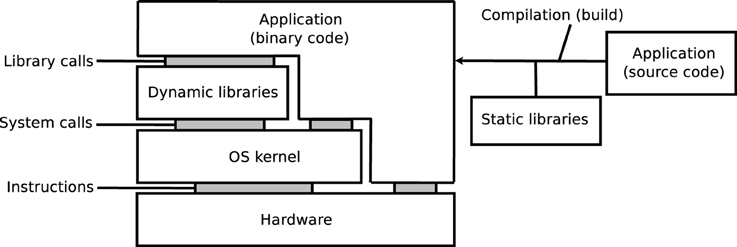
\includegraphics[width=\linewidth]{builds.jpg}
\captionof{figure}{Source code, compilation, libraries, kernel and hardware}
\label{fig:Types of builds}
\caption*{Extracted from \cite{Gla15}}
\end{center}

%Gronenschild study summary
The above studies point out the reasons that can cause differences in the output images. The difference in the output images due to updates, compilation process, software library version, kernel version or the architecture of the hardware it uses for execution are some of the main reasons. With the use of containers, the variance in these reproducibility issues can be minimized to a certain extent. We focus on the reproducibility aspect of HCP pipelines across operating systems, like how stable the pipeline is, if the results are different across operating systems, quantify them and find the reason behind the differences.

\section{Containers}
%Containers intro
A container is a self-contained, ready-to-use software component with all the necessary dependencies and softwares~\cite{7158965}. Containers allow a user to run an application and its dependencies in resource-isolated processes by encapsulating the entire software environment. Containers thus help in tackling one of the serious challenges associated with making an experiment computationally reproducible, i.e., the rapidly changing nature of computer environments.
%2 History of containers
% Clone and snapshot
% Clone and snapshot explanation
% Open solaris - name
% Describe open VZ
% What is namespace
% LXC
% Combine lxc, add namespace.
% Continaers instead of continaer based 
% Explain iptable 
The container technology has been around for a while and there are numerous implementations of it. In the year 2000, FreeBSD (4.0) featured the Jails system which focused on providing a virtual environment running on the host machine with its own files, processes, user and superuser accounts. Later came Solaris Containers, providing not only isolation services but also mechanisms related to snapshot and cloning. A snapshot is a read-only copy of a file system or volume while a clone is a writable volume or file system created from a snapshot. In 2005, OpenVZ\footnote{\url{https://openvz.org/Main_Page}} was announced as a containerization technology supporting Linux systems and Virtuozzo\footnote{\url{https://openvz.org/Virtuozzo}} containers was built on top of OpenVZ components. Linux containers (LXC), took advantage of the namespace concept and extended its isolation property to users, processes and networking. Linux Programmer's Manual~\cite{namespaces} describes namespace as, ``a global system resource in an abstraction that makes it appear to the processes within the namespace that they have their own isolated instance of the global resource". In 2006, Google started a project which implemented a functionality to limit the resource usage of containers. This project was later merged into the Linux kernel and it was named as ``cgroups" feature. Linux Programmer's Manual~\cite{cgroups} defines cgroup as, ``Control cgroups, usually referred to as cgroups, are a Linux kernel feature which allows processes to be organized into hierarchical groups whose usage of various types of resources can then be limited and monitored". Docker, was started as an open source project in 2013, which basically added an additional layer on top of Linux Containers (LXC), exposing additional features such as mounted storage, network port redirection, and container catalog management. Singularity, was started in 2015, with focus on experimental reproducibility and isolation~\cite{Xavier:2013:PEC:2497369.2497577}.

%Different kinds of virtualization
Full virtualization, paravirtualization and containers are different kinds of virtualization. In full virtualization, guest operating systems can run without modifications on top of the host operating system and the virtual machine monitor (VMM)~\cite{7382987}. According to~\cite{hypervisor}, ``Hypervisor also known as Virtual Machine Monitor, is the basic software for providing virtualization. Virtualization creates the environment for various operating system to run on a single node or host computer or machine. The main purpose of the hypervisor is to monitor the Virtual Machine (VM) that runs above the VMM. This enables more than one guest machine to utilize the hardware resources of a single host machine". In paravirtualization, the guest OS (the one being virtualized) is aware that it is in a virtualized environment and the guest's kernel is modified to communicate directly with the virtualization hypervisor~\cite{7382987}. OS-Layer virtualization or container-based virtualization differs from full or paravirtualization by modifying the underlying OS to isolate instances. It utilizes host OS kernel to provide isolation and multi-tenancy layer.

\begin{center}
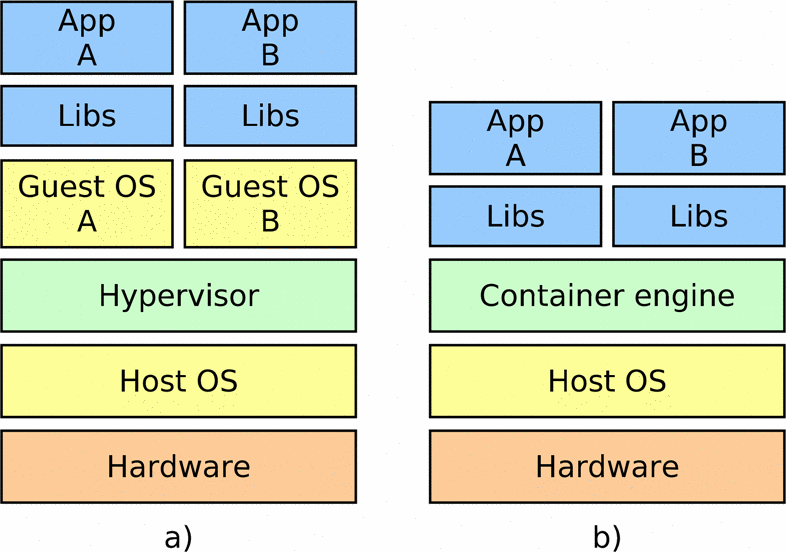
\includegraphics[width=\linewidth]{cont-vm.png}
  \captionof{figure}[Comparison of hypervisor and container]{Comparison of hypervisor-based (a) and container-based (b) instances.}
\label{fig:Comparison of container vs. hypervisor}
\caption*{Extracted from \cite{7382987}}
\end{center}

%Differences container and virtual machine 
Figure \ref{fig:Comparison of container vs. hypervisor} illustrates the differences based on hypervisor and container. Containers have a closer access to operating system services than their counterpart virtualization tools which makes their performance closer to the performance exhibited on top of native environments~\cite{Xavier:2013:PEC:2497369.2497577}. Containers access the host operating system directly, which reduces the overhead compared to other types of virtualization.

% Features of containers
Some of the notable features of containers~\cite{docker-run}~\cite{DBLP:journals/corr/HaleLRW16}~\cite{Julian:2016:CRI:2949550.2949562}~\cite{10.1109/ISPASS.2015.7095802} which facilitate conducting experiments easily are listed below:

\begin{itemize}
  \item Helps in encapsulating the entire software environment.
  \item Avoids the software version conflicts with the host OS by packaging the right software versions and dependencies in the container environment.
  \item Simplifies collaboration and sharing ability.
  \item Improves reproducibility and portability of applications.
  \item Facilitates the rapid deployment and execution at scale.
\end{itemize}

%\todo{Write this: What are its limitations. Introduce and comment on the table.}

However, containers are not the ultimate solution for reproducible computations. Reproducibility issues may arise from other causes than software libraries, for instance amount of available resources or hardware heterogeneity, which are not covered by containers. Table~\ref{tab:table_docker} shows the various issues found while using Docker containers.
%Include the problems listed in link https://goo.gl/zodrok

\begin{center}
\tabulinesep=1.2mm
\begin{tabu} to \textwidth { | X[l] | X[l] | X[l] | X[l] |}
  \hline
  \textbf{Error type} & \textbf{Cause} & \textbf{Software} &  \textbf{Solved by containers?} \\
  \hline
  Numerical differences & OS libraries & FSL, Freesurfer, CIVET & Masked \\
  \hline
  Numerical differences & Unnoticed crash & FSL (epi\_reg) & Depends on crash cause \\
  \hline
  Crash & Hardware-specific instructions & MRtrix3 (default compilation options have architecture-specific compilation flags) & No \\
  \hline
  Crash & Out of memory & FSL (applywarp) & No \\
  \hline
\end{tabu}
\captionof{table}{Container Issues}
\label{tab:table_docker}
\end{center}

%Numerical issues in containers
Containers help in reducing the variability in the images caused due to the numerical instability of pipelines. The differences found in FSL, FreeSurfer and CIVET are actually masked by the use of containers, since, the condition on which the processing takes place doesn't change if we are using the same container image. If the image gets updated, the results might be different.

Niak\footnote{\url{http://niak.simexp-lab.org/niak\_pipelines.html}} is a preprocessing pipeline consisting of tools for the connectivity analysis in fMRI. Niak pipeline has numerical instability stemming from the differences in the host kernel used by the container. 

MRtrix3\footnote{\url{http://www.mrtrix.org/}} is a set of tools to analyze the diffusion MRI data. MRtrix3 has architecture specific compilation flags. Therefore, the application seems to crash when it is executed on a hardware with different architecture.

\subsection{Pipeline Containerization}
Figure~\ref{fig:container_architecture} illustrates the container image architecture. The architecture is based on LXC which makes use of cgroups and namespaces. The images are layered on top of each other and the writable container image is kept at the top. The top layer is executable and it can have a state. The container can be considered as a directory containing everything needed for execution of an application~\cite{7158965}.\\

\begin{center}
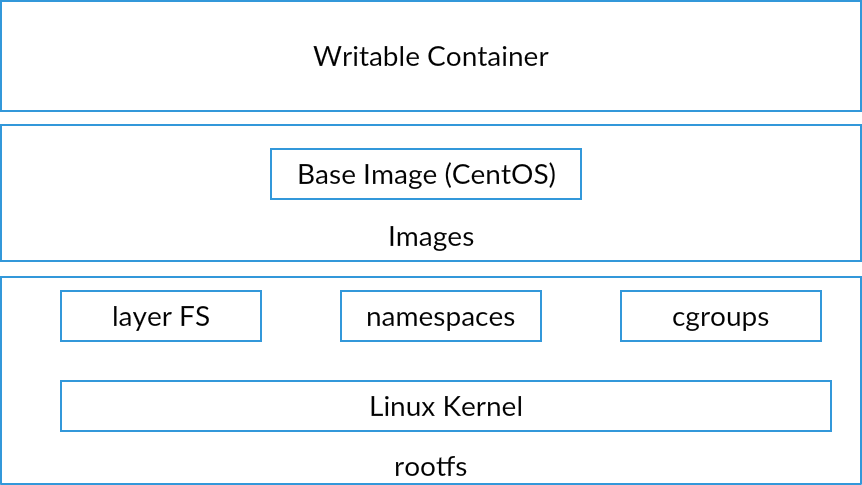
\includegraphics[width=\linewidth]{container_architecture_unedit.png}
\captionof{figure}{Container Architecture}
\label{fig:container_architecture}
\end{center}

Namespace isolation prevents processes from seeing resources allocated to each other. Container technologies use separate namespaces dedicated for each functionality, such as, process isolation, network interfaces, interprocess communication etc. Control groups manage and limit resource access for process groups through limit enforcement, accounting and isolation. Thus, namespace and cgroups makes it easier to manage and execute multi-tenant containers on the host system.

\subsection{Docker}
%Docker intro
As illustrated in Figure~\ref{fig:docker_architecture}, Docker uses a client-server architecture. The Docker software runs as a daemon on host machine. This daemon can launch containers, control their isolation level, monitor them to trigger actions, and spawn shells into running containers for administration purposes. Daemon can change firewall rules on the host and create network interfaces. Docker can create and store images encapsulating an entire software environment. Docker images can be stored locally or it can be stored in Dockerhub\footnote{\url{https://hub.docker.com/}}. Dockerhub is an online repository that helps developers to manage the Docker images. Anyone who sign up on the Dockerhub has access to public images, and they can also host their own images. There is also feature to automate the image creation with the help of Git\footnote{\url{https://git-scm.com/}}. Any user can create repository under his account and the repositories are namespaced using the format, "\textless developer\textgreater/\textless repository\textgreater"~\cite{7742298}. The management of the images on the host machine, pushing and pulling of images from Dockerhub\footnote{\url{https://www.hub.docker.com/}}, building images from Dockerfile are all taken care by the daemon. The daemon itself runs as a root user on the host machine and it is remotely controlled through a Unix socket. The Docker client talks to the Docker daemon and the daemon does all the heavy lifting like pushing, pulling and building images. The Docker client and daemon communicate using a REST API, over UNIX sockets or a network interface. The client and daemon need not necessarily be on the same machine~\cite{docker-documentation}.

\begin{center}
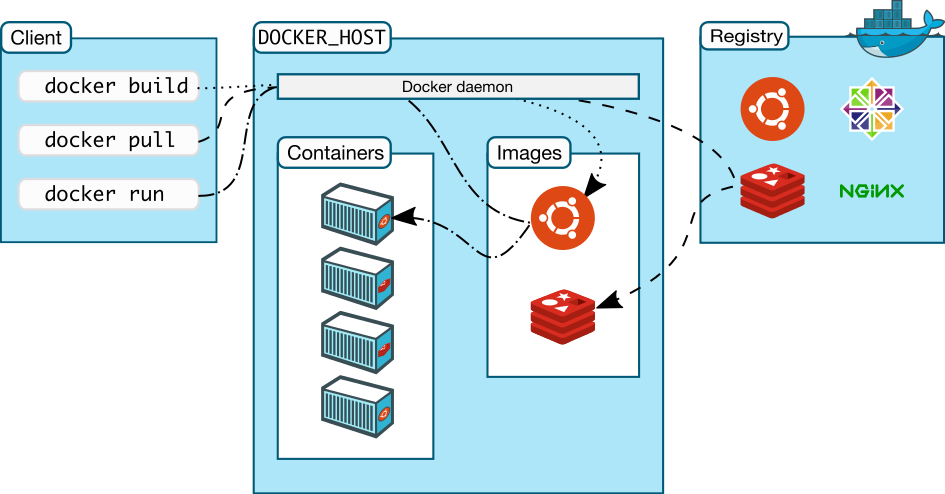
\includegraphics[width=\linewidth]{docker_architecture.png}
\captionof{figure}{Docker Architecture}
\label{fig:docker_architecture}
\caption*{Extracted from \cite{docker-documentation}}
\end{center}

%Docker ianges docker hub iwth or
% Anyone who signs up
% Explain dockerfile sample
%Docker Features

Docker provides access to virtualization facilities provided by the Linux kernel, along with some abstracted virtualized interfaces such as libvirt\footnote{\url{https://libvirt.org/}}, LXC and systemd-nspawn\footnote{\url{https://www.freedesktop.org/software/systemd/man/systemdnspawn.html}}. The control over the host's resources is provided thorough Control Groups (cgroups) and thus it limits the amount of resources used by a container such as memory, disk space and I/O. Docker features a layered file system called AuFS (Advanced Multi Layered Unification File System) which allows to overlay one or more existing file systems. AuFS feature provides capabilities such as image versioning management and exposing base images to more specialized virtualized systems. One of the main reason for the wide adoption of Docker containers is that it can leverage the infrastructure consolidation (an organization's strategy to reduce IT assets by using more efficient technologies) and it exhibits a low resource footprint. Docker also boosted the adoption of service oriented architectures (e.g. micro services) because that makes the deployment of self-contained modules easy. They are also able to independently interact with third parties using existing network protocols (e.g. web services)~\cite{Xavier:2013:PEC:2497369.2497577}. 

\begin{center}
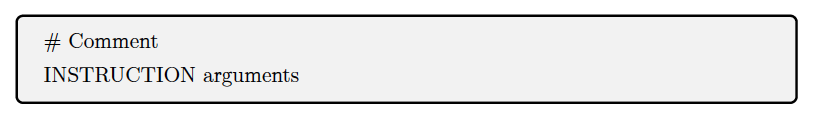
\includegraphics[width=\linewidth]{docker_sample_format}
\captionof{figure}{Docker Sample Format}
\label{fig:docker_format}
\end{center}

\begin{center}
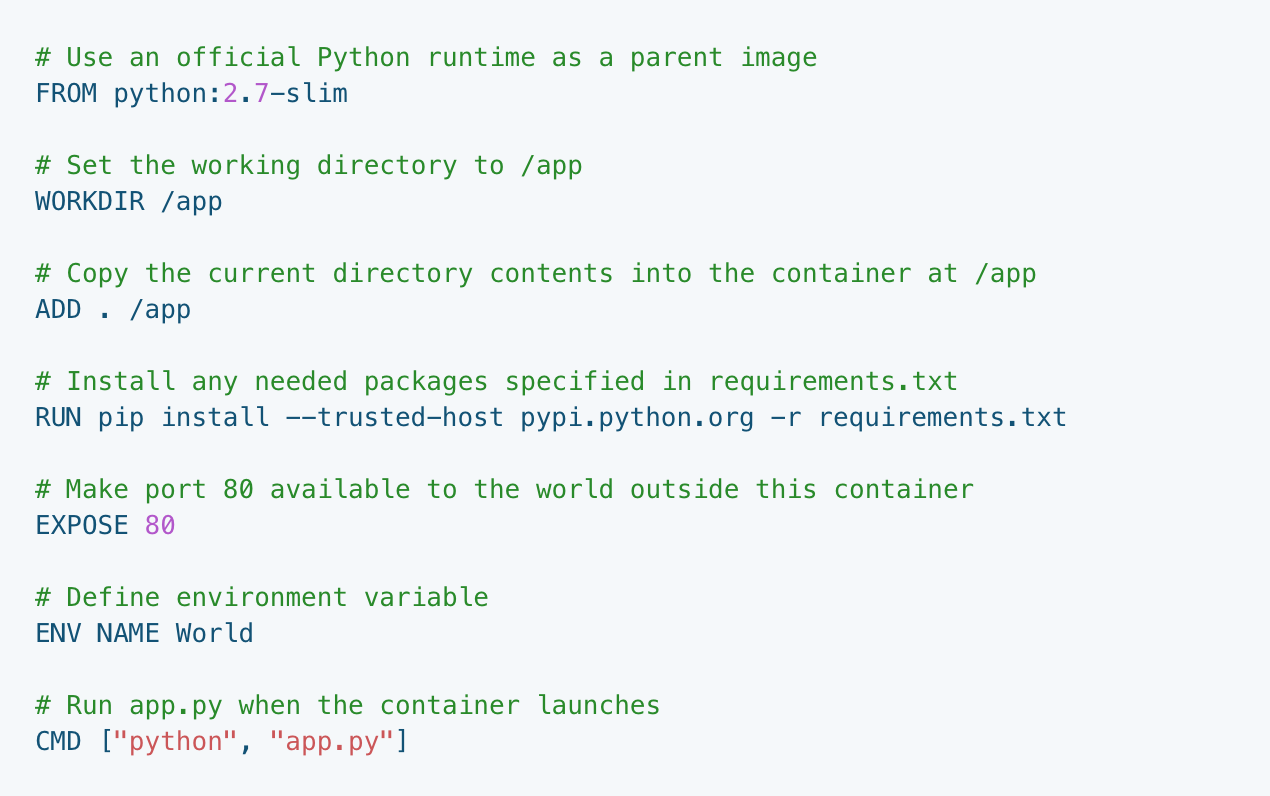
\includegraphics[width=\linewidth]{Docker_Sample_File}
\captionof{figure}{Docker Sample File}
\label{fig:docker_file_format}
\caption*{Extracted from \cite{docker-file-format}}
\end{center}

%Docker build commands
The sample file format of a Dockerfile is shown in Figure~\ref{fig:docker_format}. The development of standardized Dockerfile format as illustrated in Figure~\ref{fig:docker_file_format}, for describing and managing software containers is very straightforward. FROM keyword is used to mention the parent image name. WORKDIR sets the current working directory and ADD helps to copy files or directories. RUN is used to run a specific command and EXPOSE keyword helps to open ports for access outside the container. ENV command is used for setting the environment variables and CMD command helps us to run scripts along with its arguments. There are many more commands and the complete documentation is available at~\cite{docker_commands}.

%How it helps run experiments
Docker helps developers to easily create standard containers for their software applications or services. For a system administrator, Docker helps in the automation of deployment and management of business level services with the help of containers. Docker can be used as a part of virtualization layer for deploying and managing the execution environments. Another advantage is that Docker containers provide reliable and predictable execution environments and thus helps in reducing the issues related to deployment~\cite{DBLP:journals/corr/MorrisVHM17}.

\subsection{Singularity}
%Singularity intro
According to~\cite{10.1371/journal.pone.0177459}, ``Singularity is an open source initiative that harnesses the expertise of system and software engineers and researchers alike, and integrates seamlessly into common workflows for both of these groups. One of the major reason for this open source initiative started by the Lawrence Berkeley National Laboratory (LBNL) was that, if Docker is used on HPC environments, that would mean an unreasonable level of security risk. So Docker could not be used by a large group of people that needed it greatly. Thus, Singularity open source initiative came up with a product that could be used across academia and industry which is agnostic to the environment. It was developed in collaboration by HPC administrators, developers and research scientists alike. The main issue with docker running on the HPC clusters was that the daemon has to run as a root user which could lead to unnecessary risks like coercing the daemon process into granting the users escalated privileges".

\begin{center}
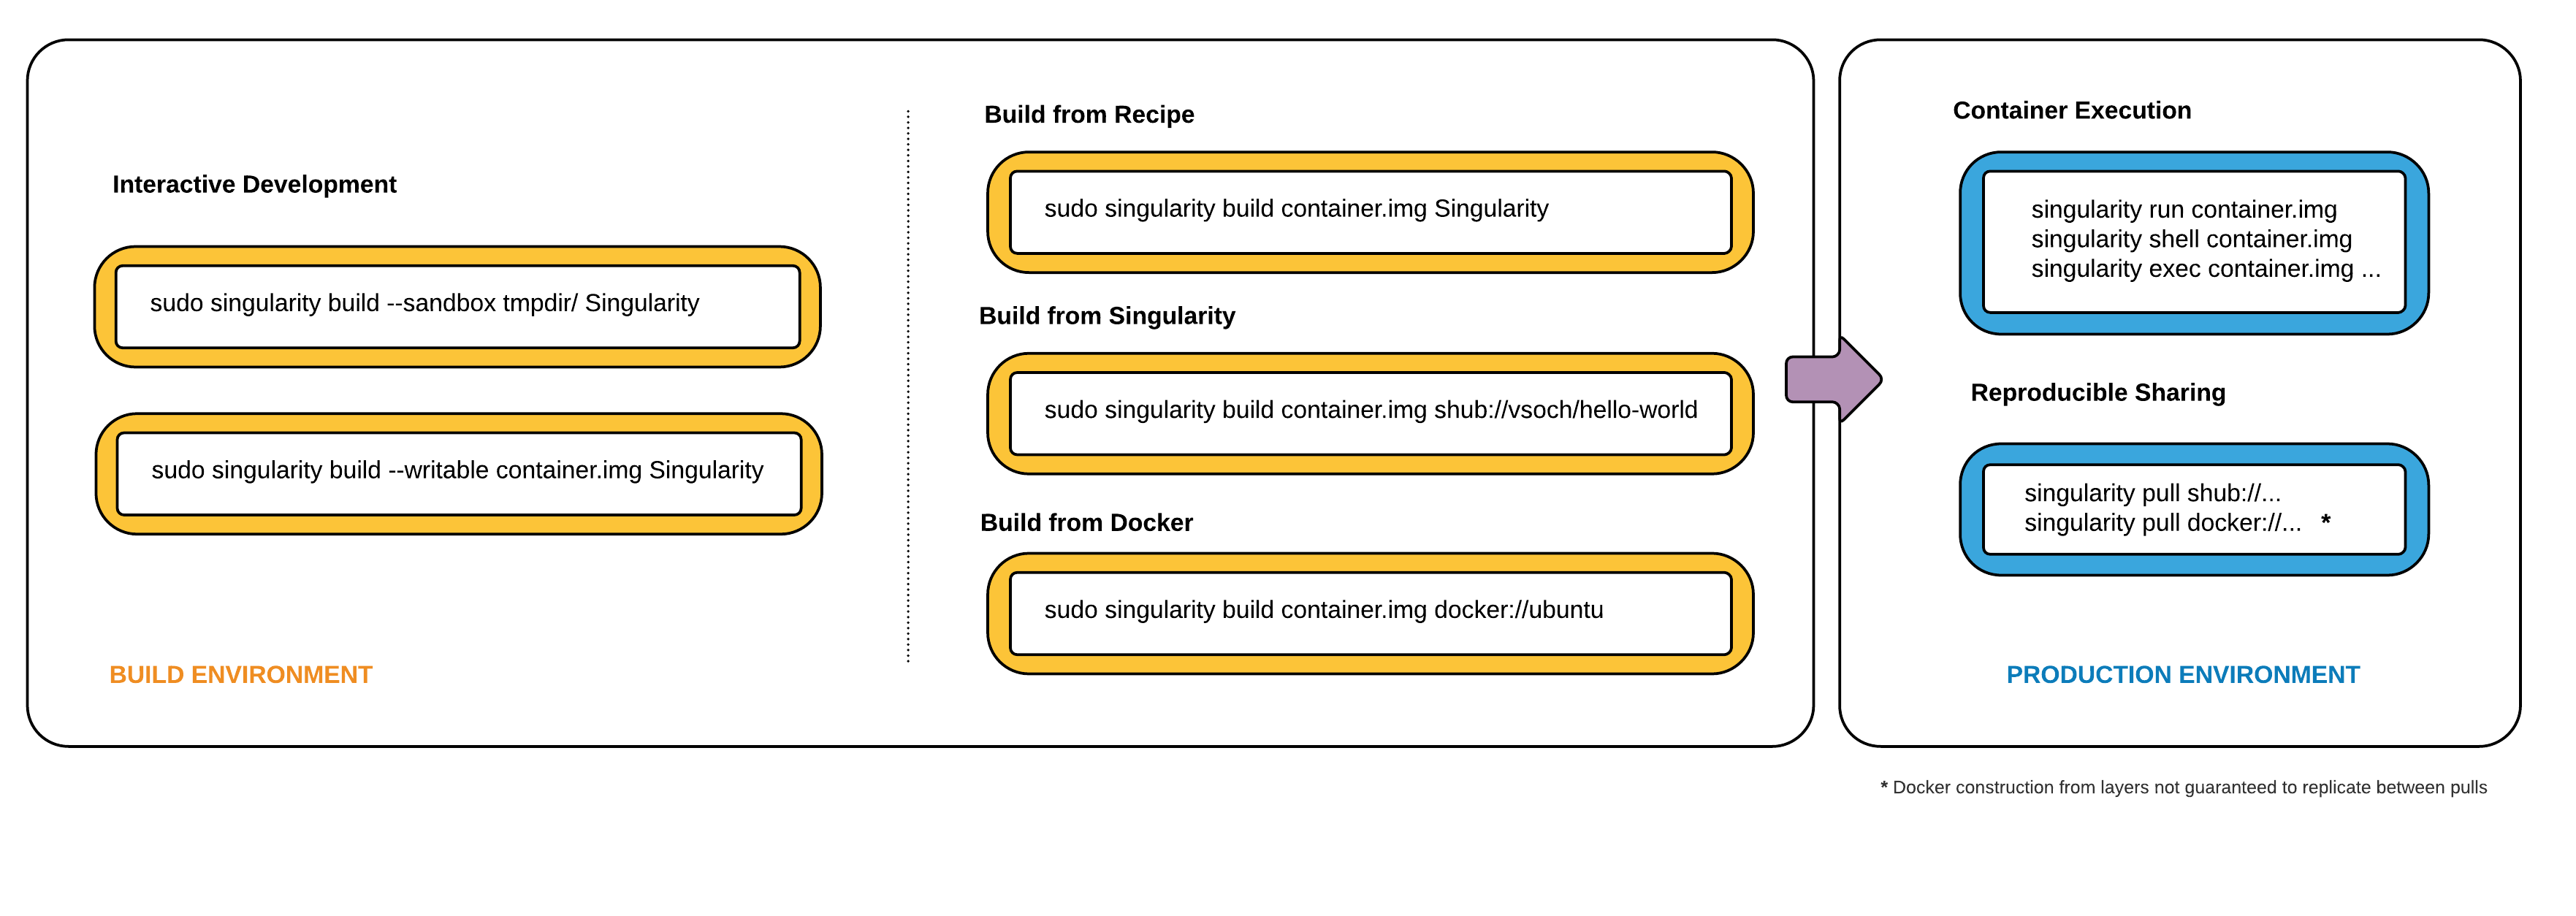
\includegraphics[width=\linewidth]{singularity.png}
\captionof{figure}{Singularity usage workflow.}
\label{fig:singularity_workflow}
\caption*{Extracted from \cite{10.1371/journal.pone.0177459}}
\end{center}
%Singularity feature
% Add spaces after bracket
% Add nextflow paper

The main goals of Singularity are, 1) Mobility of compute 2) Reproducibility 3) User Freedom 4) Support on existing traditional HPC resources. According to~\cite{10.1371/journal.pone.0177459}, ``Mobility of compute is defined as the ability to define, create, and maintain a workflow locally while remaining confident that the workflow can be executed on different hosts, Linux operating systems, and/or cloud service providers". Singularity achieves this by utilizing a distributable image format that encapsulates the entire container and stack into a single image file. The feature that supports reproducibility is the use of hashing. Any singularity image can make use of the hash feature to create hash and store it as metadata with built images. Users can verify these hashes to check if the image is modified or not. User freedom is granted by the ability to define their own working environment and copy the Singularity image containing the entire details of that environment along with the code to a shared resource and reproduce the workflow inside that image. Singularity supports the existing and traditional HPC resources easily as installing a single package onto host operating system. Singularity is compatible with RHEL and Linux distributions dating back to Linux2.2. It natively supports the resource managers (e.g SLURM\footnote{\url{https://slurm.schedmd.com/}} - a free and open-source job scheduler for Linux and Unix-like kernels, Torque\footnote{\url{http://www.adaptivecomputing.com/products/open-source/torque/}} - an open-source Resource and QUEue Manager is a distributed resource manager providing control over batch jobs and distributed compute nodes, SGE\footnote{\url{https://en.wikipedia.org/wiki/Oracle_Grid_Engine}} - a grid computing computer cluster software system, etc.) and supports technologies such as InfiniBand\footnote{\url{https://en.wikipedia.org/wiki/InfiniBand}}(A computer-networking communications standard used in high-performance computing that features very high throughput and very low latency) and Lustre\footnote{\url{https://en.wikipedia.org/wiki/Lustre_(file_system)}}(Open source, parallel file system that supports many requirements of leadership class HPC simulation environments).

%Singularity how it helps
Singularity image encapsulates the operating system environment and all application dependencies necessary to run a defined workflow. Singularity container supports different kinds of uniform resource identifiers (http:// and https://) and also other container formats like Docker (docker:// - for pulling images from docker hub, shub:// - for pulling images from singularity hub). Singularity images thus can be created from existing Docker images.

\section{Web platforms and tools to run containers}
%\subsection{Why do we need these platforms?}
\subsection{Examples of web computing platforms}
%How do you put neuro into clusters and how do you scale.
% Move boutiques to 2.3 
\subsection{CBRAIN}
%CBRAIN OVerview
% Cite paper
The Canadian Brain Imaging Research Platform (CBRAIN), is a web platform developed at the Montreal Neurological Institute (MNI) to tackle the Big-Data research and heavy computational challenges faced by neuroimaging researchers. Even though it is mainly used for neuroimaging, the framework is so generic that it can work on data and tools irrespective of discipline~\cite{DBLP:journals/fini/DasGRSPMSRSKMKR17}. Literature on CBRAIN~\cite{DBLP:journals/fini/DasGRSPMSRSKMKR17} defines the platform as, ``a controlled and secure platform which is user-friendly, lightweight, extensible and it can support heterogeneous computing platforms and data resources. It also provides access to an array of processing and visualization tools". The CBRAIN service deployed at the Montreal Neurological Institute relies on the infrastructure provided by Compute Canada~\cite{DAS20161188}. It currently provides 500+ collaborators in 22 countries with web access to several systems, including 6 clusters of Compute Canada\footnote{\url{https://www.computecanada.ca/}} high-performance computing infrastructure (totaling more than 100,000 computing cores and 40 PB of disk storage) and Amazon EC2. CBRAIN transiently stores about 10 million files representing over 50 TB distributed in 42 servers. 51 public data processing applications are integrated and over 340,000 processing batches have been submitted since 2010.

%CBRAIN Architecture brief intro
According to~\cite{DBLP:journals/fini/DasGRSPMSRSKMKR17} three main layers of CBRAIN are, `` (i)the access layer, accessible through a standard web-browser (for users) or a RESTful WebAPI (for applications or other platforms), (ii) the service layer which provides portal services for the access layer, the metadata database, which stores information about all users, permissions, and resources, and orchestration services for resource coordination (users requests, data movement, computing loads, jobs, data models, ...), and finally (iii) an infrastructure layer consisting of networked data repositories and computing resources".

%CBRAIN support containers and Boutiques
CBRAIN supports container technologies like Docker, Singularity and it also extends its support to Boutiques. Thus, with the help of container technologies and Boutiques, applications can be ported to CBRAIN. Any user who has access to this application can try to reproduce the experiments since the data and the application are accessible within the framework. However, one caveat is that, the neuroimaginng pipelines might have different results due to differences in computing platforms on which the images are getting processed ~\cite{10.3389/conf.fninf.2014.18.00076}.

The components of CBRAIN are implemented using Ruby on Rails, a widely used RESTful, Ruby based framework. Ruby classes are used for integrating applications into the platform and those classes can create web forms which creates the user interface for the application, validate the parameters and helps in running the command lines. These user interfaces are created out of standard templates and thus it helps in having uniformity across the application interfaces with respect to the user experience.

Applications into CBRAIN can be integrated in two ways. (i) The descriptor is stored in a CBRAIN plugin and the Ruby classes are generated when the CBRAIN server starts. But this mode has the limitation that it does not allow for customization beyond the Boutiques schema. (ii) Second mode generates Ruby classes through an offline process and it allows developers to customize the application by editing these Ruby classes. However, one caveat in using this mode is that manual intervention is needed whenever the descriptors get updated to update these classes.

\subsection{Amazon}
%AWS Intro
Amazon Web Services\footnote{\url{https://aws.amazon.com/}} (AWS) offers cloud computing services. The white paper on AWS~\cite{Amazon-Web-Services} states that, ``Cloud computing is the on-demand delivery of compute power, database storage, applications, and other IT resources through a cloud services platform via the Internet with pay-as-you-go pricing"~\cite{Amazon-Web-Services}. One of the main advantages of cloud computing is that it can eliminate the need for up-front capital for infrastructure as businesses can leverage the scale of computing according to the demand and thus save significant amount of money. Cloud computing models\footnote{\url{https://aws.amazon.com/types-of-cloud-computing/}} of three types (i) Infrastructure as a Service (IaaS), provie access to networking features, computing infrastructure and data storage capability. (ii) Platform as a Service (PaaS), offers complete management of the infrastructure including resource procurement, planning, maintenance, patching etc. (iii) Software as a Service (SaaS), provides completed product that is run and managed by the service provider. There are a variety of cloud-platform services provided by AWS. Elastic Compute Cloud (EC2) and Simple Storage Service (S3) are the most popularly used ones in terms of computing and storage.

%Amazon EC2
EC2 provides you total control over the virtual machines (instances) which you can create and you have to pay according to the resources that you actually use. Each virtual machine configuration that a user can create from the AWS user interface is called an "instance type". The pricing strategies of EC2 are of three kinds: (i) On Demand Instances - where you pay for compute capacity by the hour. (ii) Reserved instances - where you have the flexibility to change families, OS types etc and also a significant discount (up to 75\%). (iii) Spot Instances - where users are allowed to bid on spare EC2 computing capacity. If the bid amount goes higher than the bid price by the user, the instance is terminated instantly.

%Amazon S3
The white paper~\cite{Amazon-Web-Services} claims that, ``Amazon S3 is object storage built to store and retrieve any amount of data from anywhere on the web". The downloading of data from S3 incurs a charge, but transferring data to S3 is free. S3 is thus suitable for less frequently accessed data.

%What it offers
In neuroimaging, processing of datasets are done using complicated pipelines that are both time-consuming and computationally intensive. Pipelines might even run for days, depending upon the type and size of dataset. The image size also can increase exponentially due to the processing through pipelines. The total cost of owning the infrastructure for processing these sorts of data increases non-linearly with processing requirements. The ability of cloud computing services to create a cluster on demand would thus help neuroimaging research to tackle larger problems.

\subsection{Boutiques}
To enable sharing of ideas and software, it is a common practice to port the applications to common platforms so that the community as a whole is able to make use of the ready-to-use applications. However, porting applications to a high performance computing infrastructure or a web platform is not so easy. Application porting needs considerable effort of manual effort to `` 1) install the application on the target infrastructure, 2) describing the application in a format compatible with the execution platform, and 3) generating proper user interfaces"~\cite{boutiques}. These installations and deployments are platform specific and thus the same tasks has to be repeated from one platform to another. Boutiques, an open source tool, can be used to save time and cost spent on these repeated actions to deploy applications on various platforms.

According to ~\cite{boutiques}, ``Docker and Singularity, greatly facilitate the sharing of software and improve the reproducibility of analysis by defining immutable, reusable execution environments". The software or applications inside these containers should be invoked through proper command line to run an application. Boutiques makes use of a flexible template that could properly describe the inputs and outputs an application produces. ``The formal descriptions, also known as \textit{manifests}, are used for validation of input values to prevent errors. These manifests are intended to be produced by scientific application developers, for publishing them in common repositories and to be consumed by execution platforms". The preferred way of describing these command line template, input and argument is through a JSON document. The manifest contains the details to a container where the intended application is installed. The proper command line argument is built at runtime with the help of manifest and the template gets replaced by the actual values given by the user. For validating the inputs an invocation schema is used.

Here is an example of a typical command-line template:

\begin{verbatim}
          exampleTool [INPUT-FILE] [OUTPUT_FILE]
\end{verbatim}

The command line above invokes a tool named exampleTool that needs two arguments, an input file and an output-folder. ``\textit{Inputs} must have a name, a unique identifier and a type. They may be optional, have a description, a value key, a flag separator, and a default value. Inputs may also be ordered lists: in this case, value keys are substituted by the space-separated list of input values. \textit{Output} files must have a unique identifier, a name and a path template that specifies the file or directory name"~\cite{boutiques}.

At runtime, with the help of the JSON descriptor, Boutiques substitutes all the mandatory parameters and the optional parameters with the original values selected by the user. The core tools of Boutiques are validator and local executor. Boutiques validator checks if the JSON manifests confirm to the rules of Boutiques schema. And local executor can be used to test and debug the applications locally.

\begin{center}
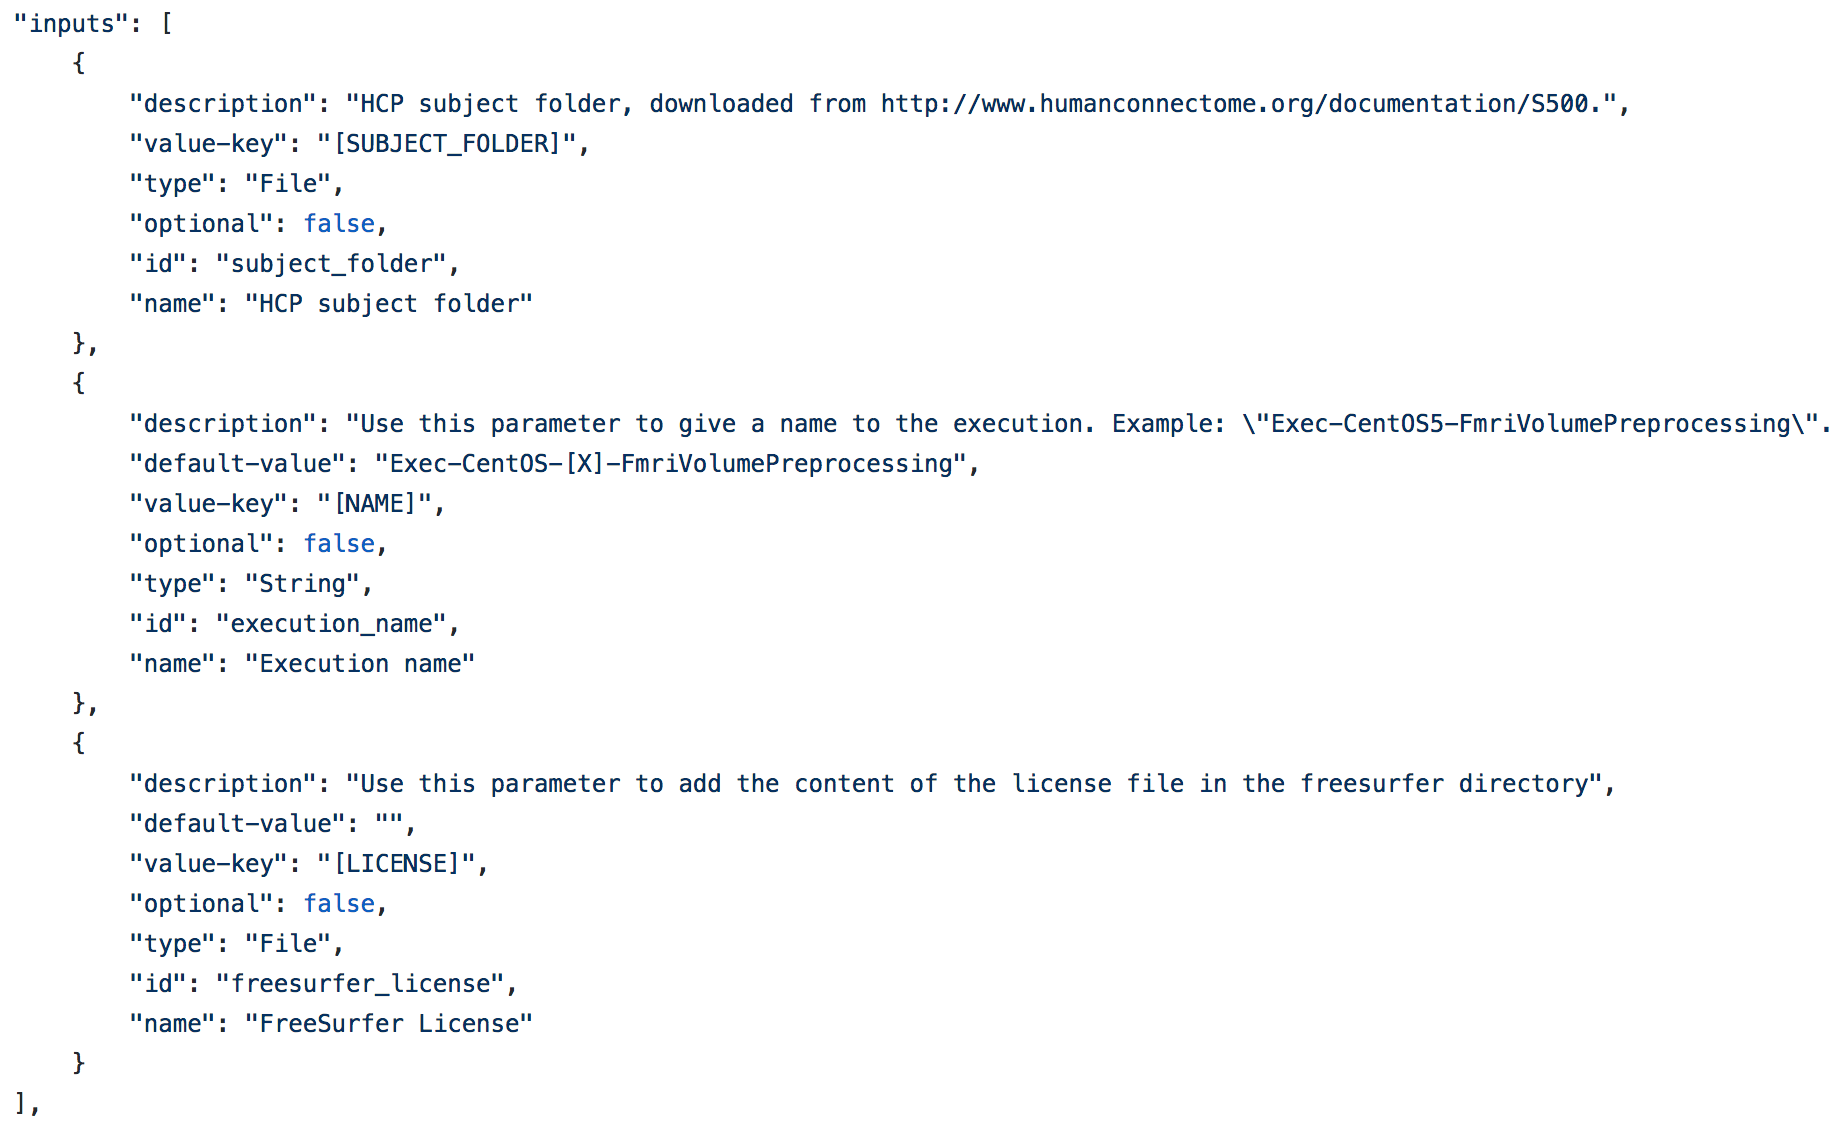
\includegraphics[width=\linewidth]{input.png}
\captionof{figure}{Boutiques input descriptor.}
\label{fig:input}
\end{center}

\begin{center}
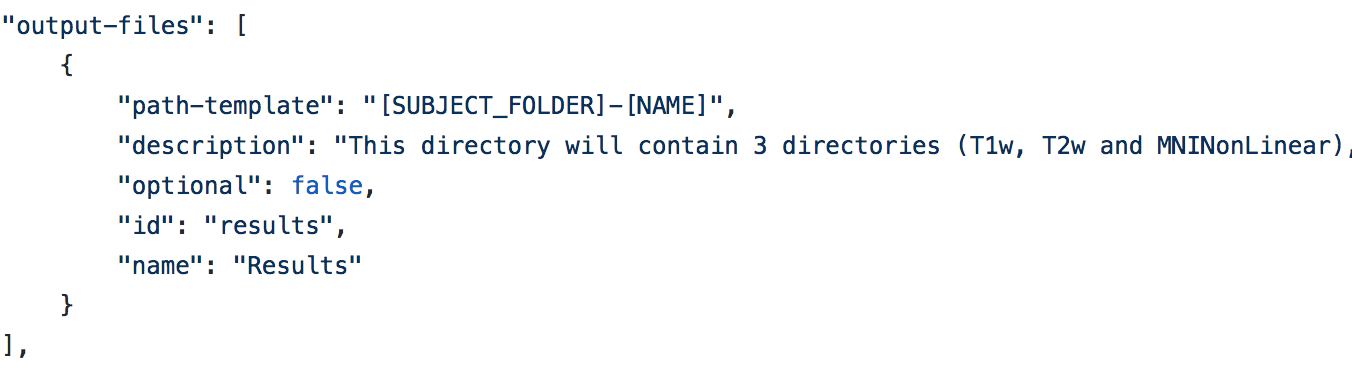
\includegraphics[width=\linewidth]{output.png}
\captionof{figure}{Boutiques output descriptor.}
\label{fig:output}
\end{center}

\section{Interposition Techniques}

\subsection{System and Library call interposition}
System call interposition is a mechanism that allows a process to monitor the system calls made by another process~\cite{Jain00user-levelinfrastructure}. System call interposition techniques can be used to implement several important features such as 1) system call tracing and monitoring, 2) the emulation of other system call implementations, 3) wrapper environment for testing untrusted binaries, 4) transactional software environments which keeps track of all the operations and can record a commit or abort message based on the transactions etc. \cite{Jones93}.

Library call interposition techniques are used for monitoring and logging the calls made to the shared libraries by different applications or processes. According to~\cite{Curry:1994:PTD:1267257.1267275}, ``The process of placing a new or different library function between the application and its reference to a library function", is called library call interposing. This technique uses wrapper functions which are modified to collect information before and after calling the real library function and thus it doesn't require to modify either the library or the application.

One of the main application where interposition technique gets used is for debugging. In Linux, utilities like gdb\footnote{\url{https://www.gnu.org/software/gdb/}}, strace\footnote{\url{https://linux.die.net/man/1/strace}}, ltrace\footnote{\url{http://man7.org/linux/man-pages/man1/ltrace.1.html}} and ptrace\footnote{\url{http://man7.org/linux/man-pages/man2/ptrace.2.html}} are used for debugging by tracing the system processes and library calls. Ptrace system-call interface is explicitly used for tracing processes~\cite{Keniston_ptrace}. The most widely used debugger in Linux, ``gdb" uses the help of ptrace to control the program to be debugged, ``strace" utility used for system call tracing makes use of ptrace's PTRACE\_SYSCALL feature and ``ltrace" utility used for tracing the dynamic library function calls also uses ptrace features~\cite{Keniston_ptrace}.

\subsection{Reprozip tool}
%What is reprozip
Reprozip\footnote{\url{https://reprozip.readthedocs.io/en/1.0.x/reprozip.html}} is a tool to make computational experiments reproducible across different platforms~\cite{Chirigati:2013:RUP:2482613.2482614}. Reprozip creates a package of the whole experiment by tracking and recording all the processes and dependencies. The main two tasks of Reprozip are packing and unpacking.

%What does it do?
To package the experiment, a Linux operating system is needed but the packaged experiment can be unpacked and ran on Linux, Mac or Windows operating system. Figure~\ref{fig:Reprozip_packing_and_unpacking} illustrates the packing and unpacking steps in Reprozip. This package can be shared among the researchers so that they can test the results and thus the experiments can be reproduced.

\begin{center}
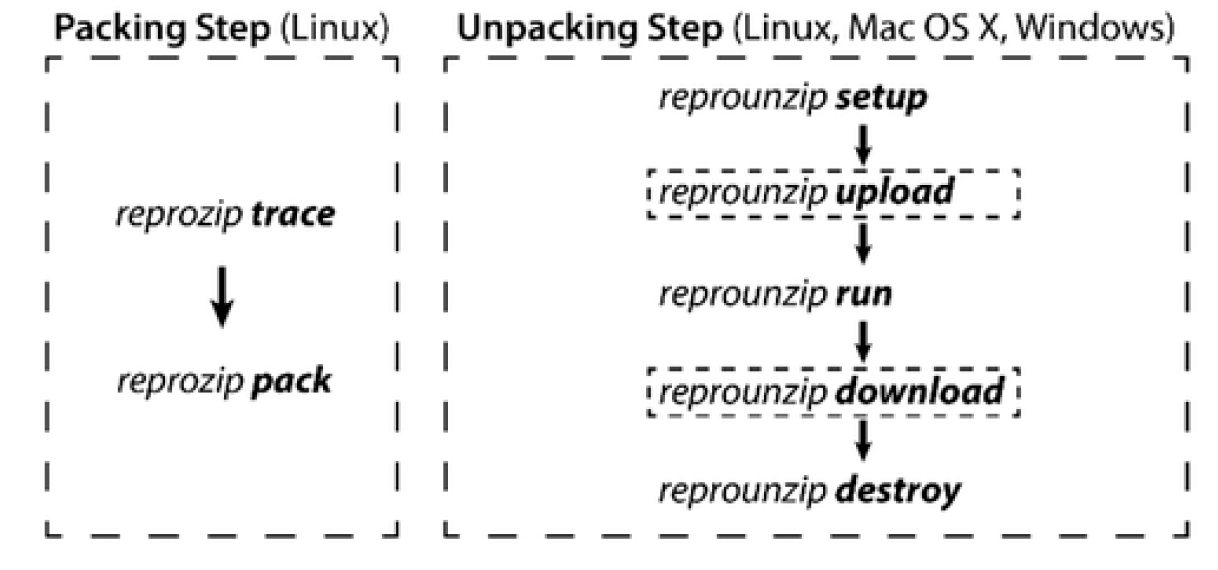
\includegraphics[width=\linewidth]{reprozip}
\captionof{figure}{Reprozip packing and unpacking}
\label{fig:Reprozip_packing_and_unpacking}
\caption*{Extracted from \cite{Rampin2016}}
\end{center}

%Packing
Reprozip uses ptrace\footnote{\url{http://man7.org/linux/man-pages/man2/ptrace.2.html}} (process trace) to trace all the system calls and hence it needs a Linux operating system for packing the experiments. The tedious task of producing a package containing all the necessary details of an experiment is made possible using four modules. System Call Tracing, Provenance Analysis, Package Customization, and Package Generation~\cite{Chirigati:2013:RUP:2482613.2482614}. Tracing includes command-line arguments, environment variables, files read, and files written, and stores everything in a SQLite database. The provenance data analysis is done in order to identify the software packages, input files and output files that are used by the experiment. All these sorts of collected information is then written into a configuration file. Package customization gives the researchers the power to customize the experiment by editing the configuration files. Thus, researchers can rerun the experiment with intended changes and thus Reprozip helps to make the experiments more flexible. After tracing all the system calls, provenance analysis, optional editing of the configuration files, the experiment package can be created using the ``reprozip pack" command. The end result is a ``.rpz" file, containing all the information required for reproducing an experiment.

%Unpacking
The unpacking process makes use of the ``.rpz" file. The unpacking can be done in three ways. If the host operating system is similar to the one on which the experiment was packed, the experiment can be reproduced on the host operating system itself by installing the dependencies on the host. If the host operating system is a totally different platform, then Vagrant\footnote{\url{https://www.vagrantup.com/}} or Docker can be used to unpack and reproduce the experiment. Vagrant is a tool for the management of virtual machines in a single workflow~\cite{vagrant}. Irrespective of platforms the unpacking process consists of experiment setup and experiment reproduction steps. Experiment setup is done by calling the ``setup" command. This command copies the experiment to the intended destination and it is followed by ``run" command which reruns the experiment. The ``upload" and ``download" command can be used to replace an input file and download a processed file respectively.

%Place this better
According to~\cite{Ikeda:2010:PSP:1855795.1855800}, ``provenance captures where data came from, how it was derived, manipulated, and combined, and how it has been updated over time". Provenance information can be used to explain the source or evolution of a data set. Thus, it can help in generating a deeper understanding of the data set. It can also be used to verify and confirm that there were no bugs in the processing. Provenance information can be used to identify the bugs in the processing. It can thus, help in recomputing the steps that got corrupted and send the corrected data downstream~\cite{Ikeda:2010:PSP:1855795.1855800}
